\chapter{Implementation}
\section{Execution of get, put, list operations}
In the first section are presented in detail the implementations of the API exposed to the client, in particular are listed the steps needed to perform the operations.  In the second part  is explained the structure of the messages exchanged onto the system.

The APIs exposed to the user are:
\begin{itemize}
	\item \emph{put(key, value)}: inserts/updates the value associated with the key.
	\item \emph{get(key)}: retrieves the value associated with the key.
	\item \emph{list(ipNode)}: shows the key values pairs stored in the node with IP=ipNode.
	\item \emph{rm(key)}: removes the key and the associated value in all the node where key is stored.
\end{itemize}

\subsection{Aborting operations}
Tha \emph{Pad-fs} use a quorum system. If the quorum system is not respected,the operation are aborted.
As example during a \emph{put} operation:
\begin{•}

\subsubsection*{Get operation}
The get(k) retrieve the value associated with the key k.
The figure~\ref{fig:get} shows the steps of a successfully get operation.

\begin{figure}[H]
\centering
\includegraphics[scale=0.5]{figures/get.png}
\caption{Steps of a successfully get operation: (1) get(k). (2) selects master node for k. (3) send get message to the master node. (4) get(k) from db. (5) send get msg to READ\_NODES. (5a) get(k) from db. (6) send data to master, (7) compare (master vs backups) version (7a) if master is after than send master version to backups (7b) if master is before than store backup. (8) send reconcilied version to client. }
\label{fig:get}
\end{figure}

If get operation found conflicts among data, the conflict is resolved by the user. The master node send a \textit{ConflictMsg} to the client that expose to the user the choices.
The figure ~\ref{fig:getConflict} are shown the steps of a get operation with conflict.

\begin{figure}[H]
\centering
\includegraphics[scale=0.5]{figures/getConflict.png}
\caption{Get with conflicts:(1)get(k).(2)select master node for k (3) send get msg to master. (4)get(k) from local db. (5) ask version to Read nodes. (5a) get(k) from db. (6) send data/version to master. (7) wait at least read nodes response. (8) if concurrent versions. (8a) send msg to client with versions (9) user insert the selection. (10) send to master the selection (11) store into db and send to backups the selected version. (12) reply to client.}
\label{fig:getConflict}
\end{figure}

\subsection*{Put operation}

The figure ~\ref{fig:put} shows the steps performed by a successful put operation.
The client receives a put operation from the user, selects the master node of the key and sends the put message to the master node. The master store the new value for the key to the local database and send a copy to the backup node.

\begin{figure}[H]
\centering
\includegraphics[scale=0.5]{figures/put.png}
\caption{Steps of a successfully put operation: (1) put(k,v) from user. (2) select master node for k. (3)send put msg to master. (4) put(k,v) into local db. (5) send put msg to write nodes. (5a) put(k,v) into local db. (6) reply successful put (7) reply to client after write nodes has responded. }
\label{fig:put}
\end{figure}

\subsection*{List operation}

The figure~\ref{fig:list} shows the steps for the list operation in the system.
\begin{figure}[H]
\centering
\includegraphics[scale=0.5]{figures/list.png}
\caption{Steps of list operation}
\label{fig:list}
\end{figure}

The list operation is used to retrieve all the key value pairs stored in a node.
The client selects the master node for the key and send the list message. The node, upon the message received, gets all the key value pairs on its local database and reply to the client.


\section{Messages format}
The messages in the system are sent into UDP packets. The figure \ref{fig:msg} shows \emph{Pad-fs} message inside the payload of UDP packet. The main fields are:

\begin{itemize}
\item \textbf{ipSeder} (String) identify the ip address of the sender node of the message. 
\item \textbf{Port sender} (integer) identify the port of the sender node where the message has been sent.
\item \textbf{Type} defines the two types of messages: \textit{request} and \textit{reply} messages.
\item \textbf{OP} is the operation requested in the message. Can be one of the following: put, get, list, ok, err, dscv, rm (dscv messages are used by the client to discover nodes in the system).
\item \textbf{data} (different type) contains the payload of the message.  Can have different types, for example in a get operation the data is the String of the key.
\end{itemize}


\begin{figure}[H]
\centering
\includegraphics[scale=0.5]{figures/messages.png}
\caption{Pad-fs message}
\label{fig:msg}
\end{figure}


The messages can de divided in two subset:
\begin{itemize}
\item \textit{Application messages}: are used only to send messages from the client to the storage nodes.
\item \textit{System messages} are used only by the storage nodes  to exchange data version and control messages in the storage system.
\end{itemize}
